%beamer

% Comment/uncomment this line to toggle handout mode
\newcommand{\handout}{}

%% Beamer-Klasse im korrekten Modus
\ifdefined \handout
\documentclass[handout]{beamer} % Handout mode
\else
\documentclass{beamer}
\fi

%% UTF-8-Encoding
\usepackage[utf8]{inputenc}

\input{../framework/gbi-macros}
\usepackage[blue]{../framework/thwregex}
\usepackage{environ}
\usepackage{bm}
\usepackage{calc}
\usepackage{varwidth}
\usepackage{wasysym}
\usepackage{mathtools}


% Das ist der KIT-Stil
%\usepackage{../TutTexbib/beamerthemekit}
\usepackage[deutsch,titlepage0]{../framework/KIT/beamerthemeKITmod}
\TitleImage[width=\titleimagewd]{../figures/titlepage.jpg}
%\usetheme[deutsch,titlepage0]{KIT}

% Include PDFs
\usepackage{pdfpages}

% Libertine font (Original GBI font)
\usepackage{libertine}
%\renewcommand*\familydefault{\sfdefault}  %% Only if the base font of the document is to be sans serif

% Nicer math symbols
\usepackage{eulervm}
%\usepackage{mathpazo}
\renewcommand\ttdefault{cmtt} % Computer Modern typewriter font, see lecture slides.

\usepackage{csquotes}

%%%%%%

%% Schönere Schriften
\usepackage[TS1,T1]{fontenc}

%% Bibliothek für Graphiken
\usepackage{graphicx}

%% der wird sowieso in jeder Datei gesetzt
\graphicspath{{../figures/}}

%% Anzeigetiefe für Inhaltsverzeichnis: 1 Stufe
\setcounter{tocdepth}{1}

%% Hyperlinks
\usepackage{hyperref}
% I don't know why, but this works and only includes sections and NOT subsections in the pdf-bookmarks.
\hypersetup{bookmarksdepth=subsection} 

%\usepackage{lmodern}
\usepackage{colortbl}
\usepackage[absolute,overlay]{textpos}
\usepackage{listings}
\usepackage{forloop}
%\usepackage{algorithmic} % PseudoCode package 

\usepackage{tikz}
\usetikzlibrary{matrix}
\usetikzlibrary{arrows.meta}
\usetikzlibrary{automata}
\usetikzlibrary{tikzmark}
\usetikzlibrary{positioning}

% Why has no-one come up with this yet? I mean, seriously. -.-
\tikzstyle{loop below right} = [loop, out=-60,in=-30, looseness=7]
\tikzstyle{loop below left} = [loop, out=-150,in=-120, looseness=7]
\tikzstyle{loop above right} = [loop, out=60,in=30, looseness=7]
\tikzstyle{loop above left} = [loop, out=150,in=120, looseness=7]
\tikzstyle{loop right below} = [loop below right]
\tikzstyle{loop left below} = [loop below left]
\tikzstyle{loop right above} = [loop above right]
\tikzstyle{loop left above} = [loop above left]

% Needed for gbi-macros
\usepackage{xspace}

%%%%%%

%% Verbatim
\usepackage{moreverb}

%%%%%%%%%%%%%%%%%%%%%%%%%%%%%%%%%%%% Copy end

%% Tabellen
\usepackage{array}
\usepackage{multicol}
\usepackage{hhline}

%% Bibliotheken für viele mathematische Symbole
\usepackage{amsmath, amsfonts, amssymb}

%% Deutsche Silbentrennung und Beschriftungen
\usepackage[ngerman]{babel}

\usepackage{kbordermatrix}

% kbordermatrix settings
\renewcommand{\kbldelim}{(} % Left delimiter
\renewcommand{\kbrdelim}{)} % Right delimiter

\input{../config.tex}



% define custom \handout command flag if handout mode is toggled  #DirtyAsHellButWell...
\only<beamer:0>{\def\handout{}} %beamer:0 == handout mode

\newcommand{\R}{\mathbb{R}}
\newcommand{\N}{\mathbb{N}}
\newcommand{\Z}{\mathbb{Z}}
\newcommand{\Q}{\mathbb{Q}}
\newcommand{\BB}{\mathbb{B}}
\newcommand{\C}{\mathbb{C}}
\newcommand{\K}{\mathbb{K}}
\newcommand{\G}{\mathbb{G}}
\newcommand{\nullel}{\mathcal{O}}
\newcommand{\einsel}{\mathds{1}}
\newcommand{\Pot}{\mathcal{P}}
\renewcommand{\O}{\text{O}}

\def\word#1{\hbox{\textcolor{blue}{\texttt{#1}}}}
\let\literal\word
\def\mword#1{\hbox{\textcolor{blue}{$\mathtt{#1}$}}}  % math word
\def\sp{\scalebox{1}[.5]{\textvisiblespace}}
\def\wordsp{\word{\sp}}

%\newcommand{\literal}[1]{\textcolor{blue}{\texttt{#1}}}
\newcommand{\realTilde}{\textasciitilde \ }
\newcommand{\setsize}[1]{\ensuremath{\left\lvert #1 \right\rvert}}
\newcommand{\size}[1]{\setsize{#1}}  % Shame on you, TeXStudio...
\newcommand{\set}[1]{\left\{#1\right\}}
\newcommand{\tuple}[1]{\left(#1\right)}
\newcommand{\normalvar}[1]{\text{$#1$}}

% Modified by DJ
\let\oldemptyset\emptyset
\let\emptyset\varnothing % proper emptyset

\newcommand{\boder}{\ensuremath{\mathbin{\textcolor{blue}{\vee}}}\xspace}
\newcommand{\bund}{\ensuremath{\mathbin{\textcolor{blue}{\wedge}}}\xspace}
\newcommand{\bimp}{\ensuremath{\mathrel{\textcolor{blue}{\to}}}\xspace}
\newcommand{\bgdw}{\ensuremath{\mathrel{\textcolor{blue}{\leftrightarrow}}}\xspace}
\newcommand{\bnot}{\ensuremath{\textcolor{blue}{\neg}}\xspace}
\newcommand{\bone}{\ensuremath{\textcolor{blue}{1}}\text{}}
\newcommand{\bzero}{\ensuremath{\textcolor{blue}{0}}\text{}}
\newcommand{\bleftBr}{\ensuremath{\textcolor{blue}{\texttt{(}}}\text{}}
\newcommand{\brightBr}{\ensuremath{\textcolor{blue}{\texttt{)}}}\text{}}

% Fix of \b... commands:

\renewcommand{\boder}{\alor}
\renewcommand{\bund}{\aland}
\renewcommand{\bimp}{\alimpl}
\renewcommand{\bgdw}{\aleqv}
\renewcommand{\bnot}{\alnot}
\renewcommand{\bleftBr}{\alka}
\renewcommand{\brightBr}{\alkz}
\newcommand{\alA}{\word A}
\newcommand{\alB}{\word B}
\newcommand{\alC}{\word C}

\newcommand{\plB}{\plfoo{B}}
\newcommand{\plE}{\plfoo{E}}

\newcommand{\summe}[2]{\sum\limits_{#1}^{#2}}
\newcommand{\limes}[1]{\lim\limits_{#1}}

%\newcommand{\numpp}{\advance \value{weeknum} by -2 \theweeknum \advance \value{weeknum} by 2}
%\newcommand{\nump}{\advance \value{weeknum} by -1 \theweeknum \advance \value{weeknum} by 1}

\newcommand{\mycomment}[1]{}
\newcommand{\Comment}[1]{}

%% DISCLAIMER START 
% It is INSANELY IMPORTANT NOT TO DO THIS OUTSIDE BEAMER CLASS! IN ARTCILE DOCUMENTS, THIS IS VERY LIKELY TO BUG AROUND!
\makeatletter%
\@ifclassloaded{beamer}%
{
	% TODO 
	% no time... later.   (= never -.-)
	% redefine section to ignore multiple \section calls with the same title
}%
{
	\errmessage{ERROR: section command redefinition outside of beamer class document! Please contact the author of this code or read the F-ing disclaimer.}
}%
\makeatother%
%% DISCLAIMER END

\newcounter{abc}
\newenvironment{alist}{
  \begin{list}{(\alph{abc})}{
      \usecounter{abc}\setlength{\leftmargin}{8mm}\setlength{\labelsep}{2mm}
    }
}{\end{list}}


\newcommand{\stdarraystretch}{1.20}
\renewcommand{\arraystretch}{\stdarraystretch}  % for proper row spacing in tables

\newcommand{\morescalingdelimiters}{   % for proper \left( \right) typography
	\delimitershortfall=-1pt  
	\delimiterfactor=1
}

\newcommand{\centered}[1]{\vspace{-\baselineskip}\begin{center}#1\end{center}\vspace{-\baselineskip}}

% for \implitem and \item[bla] stuff to look right:
\setbeamercolor*{itemize item}{fg=black}
\setbeamercolor*{itemize subitem}{fg=black}
\setbeamercolor*{itemize subsubitem}{fg=black}

\setbeamercolor*{description item}{fg=black}
\setbeamercolor*{description subitem}{fg=black}
\setbeamercolor*{description subsubitem}{fg=black}

\renewcommand{\qedsymbol}{\textcolor{black}{\openbox}}

\renewcommand{\mod}{\mathop{\textbf{mod}}}
\renewcommand{\div}{\mathop{\textbf{div}}}

\newcommand{\ceil}[1]{\left\lceil#1\right\rceil}
\newcommand{\floor}[1]{\left\lfloor#1\right\rfloor}
\newcommand{\abs}[1]{\left\lvert #1 \right\rvert}
\newcommand{\Matrix}[1]{\begin{pmatrix} #1 \end{pmatrix}}
\newcommand{\braced}[1]{\left\lbrace #1 \right\rbrace}

% "something" placeholder. Useful for repairing spacing of operator sections, like `\sth = 42`.
\def\sth{\vphantom{.}}

\def\fract#1/#2 {\frac{#1}{#2}} % ! Trailing space is crucial!
\def\dfract#1/#2 {\dfrac{#1}{#2}} % ! Trailing space is crucial!

\newcommand{\Mid}{\;\middle|\;}

\let\after\circ



\def\·{\cdot}
\def\*{\cdot}
\def\?>{\ensuremath{\rightsquigarrow}}  % Fuck you, Latex
\def\~~>{\ensuremath{\rightsquigarrow}}  

\newcommand{\tight}[1]{{\renewcommand{\arraystretch}{0.76} #1}}
\newcommand{\stackedtight}[1]{\renewcommand{\arraystretch}{0.76} \begin{matrix} #1 \end{matrix} }
\newcommand{\stacked}[1]{\begin{matrix} #1 \end{matrix} }
\newcommand{\casesl}[1]{\delimitershortfall=0pt  \left\lbrace\hspace{-.3\baselineskip}\begin{array}{ll} #1 \end{array}\right.}
\newcommand{\casesr}[1]{\delimitershortfall=0pt  \left.\begin{array}{ll} #1 \end{array}\hspace{-.3\baselineskip}\right\rbrace}
\newcommand{\caseslr}[1]{\delimitershortfall=0pt  \left\lbrace\hspace{-.3\baselineskip}\begin{array}{ll} #1 \end{array}\hspace{-.3\baselineskip}\right\rbrace}

\def\q#1uad{\ifnum#1=0\relax\else\quad\q{\the\numexpr#1-1\relax}uad\fi}
% e.g. \q1uad = \quad, \q2uad = \qquad etc.

\newcommand{\qqquad}{\q3uad}
\newcommand{\minusquad}{\hspace{-1em}}

%% Placeholder utils
% \§{#1}   Saves #1 as placeholder and prints it
% \.       Prints an \hphantom with the size of the recalled placeholder.
\def\indentstring{}
\def\§#1{\def\indentstring{#1}#1}
\def\.{{$\hphantom{\text{\indentstring}}$}}
%% Placeholder utils end

\newcommand{\impl}{\ifmmode\ensuremath{\mskip\thinmuskip\Rightarrow\mskip\thinmuskip}\else$\Rightarrow$\fi\xspace}
\newcommand{\Impl}{\ifmmode\implies\else$\Longrightarrow$\fi\xspace}

\newcommand{\derives}{\Rightarrow}

\newcommand{\gdw}{\ifmmode\mskip\thickmuskip\Leftrightarrow\mskip\thickmuskip\else$\Leftrightarrow$\fi\xspace}
\newcommand{\Gdw}{\ifmmode\iff\else$\Longleftrightarrow$\fi\xspace}

% Legacy code from the algo tutorial slides. Perhaps useful. Try with care.
\mycomment{
	\newcommand{\impl}{\ifmmode\ensuremath{\mskip\thinmuskip\Rightarrow\mskip\thinmuskip}\else$\Rightarrow$\xspace\fi}  
	\newcommand{\Impl}{\ifmmode\implies\else$\Longrightarrow$\xspace\fi}
	
	\newcommand{\gdw}{\ifmmode\mskip\thickmuskip\Leftrightarrow\mskip\thickmuskip\else$\Leftrightarrow$\xspace\fi}
	\newcommand{\Gdw}{\ifmmode\iff\else$\Longleftrightarrow$\xspace\fi}
}
	
\newcommand{\gdwdef}{\ifmmode\mskip\thickmuskip:\Leftrightarrow\mskip\thickmuskip\else:$\Leftrightarrow$\xspace\fi}
\newcommand{\Gdwdef}{\ifmmode\mskip\thickmuskip:\Longleftrightarrow\mskip\thickmuskip\else:$\Longleftrightarrow$\xspace\fi}

\newcommand{\symbitemnegoffset}{\hspace{-.5\baselineskip}}
\newcommand{\implitem}{\item[\impl\symbitemnegoffset]}
\newcommand{\Implitem}{\item[\Impl\symbitemnegoffset]}


\newcommand{\forcenewline}{\mbox{}\\}

\newcommand{\bfalert}[1]{\textbf{\alert{#1}}}
\let\elem\in   % I'm a Haskell freak. Don't judge me. :P


\def\|#1|{\text{\normalfont #1}}  % | steht für senkrecht (anstatt kursiv wie sonst im math mode)


% proper math typography
\newcommand{\functionto}{\longrightarrow}
\renewcommand{\geq}{\geqslant}
\renewcommand{\leq}{\leqslant}
\let\oldsubset\subset
\renewcommand{\subset}{\subseteq} % for all idiots out there using subset

\newenvironment{threealign}{%
	\[
	\begin{array}{r@{\ }c@{\ }l}
}{%
	\end{array}	
	\]
}

\newcommand{\concludes}{ \\ \hline  }
\newcommand{\deduction}[1]{
	\begin{varwidth}{.8\linewidth}
		\begin{tabular}{>{$}c<{$}}
			#1
		\end{tabular}
	\end{varwidth}	
}

\definecolor{hoareorange}{rgb}{1,.85,.6}
\newcommand{\hoareassert}[1]{\setlength{\fboxsep}{1pt}\setlength{\fboxrule}{-1.4pt}\fcolorbox{white}{hoareorange}{\ensuremath{\{\;#1\;\}}}\setlength\fboxrule{\defaultfboxrule}\setlength{\fboxsep}{3pt}}

\newcommand{\mailto}[1]{\href{mailto:#1}{{\textcolor{blue}{\underline{#1}}}}}
\newcommand{\urlnamed}[2]{\href{#2}{\textcolor{blue}{\underline{#1}}}}
\renewcommand{\url}[1]{\urlnamed{#1}{#1}}

\newcommand{\hanging}{\hangindent=0.7cm}
\newcommand{\indented}{\hanging}


% \hstretchto prints #2 left-aligned into a box of the width of #1
\def\hstretchto#1#2{%
	\mbox{}\vphantom{#2}\rlap{#2}\hphantom{#1}%
}

\def\vstretchto#1#2{%
	\mbox{}\hphantom{#2}\smash{#2}\vphantom{#1}%
}

% \hstretchtocentered prints #2 centered into a box of the width of #1
\def\hstretchtocentered#1#2{%
	\mbox{}\vphantom{#2}\scalebox{0.5}{\hphantom{#1}}\clap{#2}\scalebox{0.5}{\hphantom{#1}}%
}

% vertical centering
\newcommand{\vertcenter}[1]{%
	\ensuremath{\vcenter{\hbox{#1}}}%
}


%requires \thisyear to be defined (s. config.tex)!
\edef\nextyear{\the\numexpr\thisyear+1\relax}


% --- \frameheight constant ---
\newlength\fullframeheight
\newlength\framewithtitleheight
\setlength\fullframeheight{.92\textheight}
\setlength\framewithtitleheight{.86\textheight}

\newlength\frameheight
\setlength\frameheight{\fullframeheight}

\let\frametitleentry\relax
\let\oldframetitle\frametitle
\def\newframetitle#1{\global\def\frametitleentry{#1}\if\relax\frametitleentry\relax\else\setlength\frameheight{\framewithtitleheight}\fi\oldframetitle{#1}}
\let\frametitle\newframetitle

\def\newframetitleoff{\let\frametitle\oldframetitle}
\def\newframetitleon{\let\frametitle\newframetitle}
% --- \frameheight constant end ---

\newcommand{\fakeframetitle}[1]{%
	\vspace{-2.05\baselineskip}%
	{\Large \textbf{#1}} \\%
	\smallskip
}



\newenvironment{headframe}{\Huge THIS IS AN ERROR. PLEASE CONTACT THE ADMIN OF THIS TEX CODE. (headframe env def failed)}{}
\RenewEnviron{headframe}[1][]{
	\begin{frame}\frametitle{\ }
		\centering
		\Huge\textbf{\textsc{\BODY} \\
		}
		\Large {#1}
		\frametitle{\ }
	\end{frame}
}


\makeatletter
% Provides color if undefined.
\newcommand{\colorprovide}[2]{%
	\@ifundefinedcolor{#1}{\colorlet{#1}{#2}}{}}
\makeatother


\colorprovide{lightred}{red!30}
\colorprovide{lightgreen}{green!40}
\colorprovide{lightyellow}{yellow!50}
\colorprovide{lightblue}{blue!10}
\colorprovide{beamerlightred}{lightred}
\colorprovide{beamerlightgreen}{lightgreen}
\colorprovide{beamerlightyellow}{lightyellow}
\colorprovide{beamerlightblue}{lightblue}
\colorprovide{fullred}{red!60}
\colorprovide{fullgreen}{green}
\definecolor{darkred}{RGB}{115,48,38}
\definecolor{darkgreen}{RGB}{48,115,38}
\definecolor{darkyellow}{RGB}{100,100,0}

\only<handout:0>{\colorlet{adaptinglightred}{beamerlightred}}
\only<handout:0>{\colorlet{adaptinglightgreen}{beamerlightgreen}}
\only<handout:0>{\colorlet{adaptinglightyellow}{beamerlightyellow}}
\only<handout:0>{\colorlet{adaptinglightblue}{beamerlightblue}}
\only<beamer:0>{\colorlet{adaptinglightred}{lightred}}
\only<beamer:0>{\colorlet{adaptinglightgreen}{lightgreen}}
\only<beamer:0>{\colorlet{adaptinglightyellow}{lightyellow}}
\only<beamer:0>{\colorlet{adaptinglightblue}{lightblue}}
\only<handout:0>{\colorlet{adaptingred}{lightred}}
\only<beamer:0>{\colorlet{adaptingred}{fullred}}
\only<handout:0>{\colorlet{adaptinggreen}{lightgreen}}
\only<beamer:0>{\colorlet{adaptinggreen}{fullgreen}}



\newcommand{\TrueQuestion}[1]{
	\TrueQuestionE{#1}{}
}

\newcommand{\YesQuestion}[1]{
	\YesQuestionE{#1}{}
}

\newcommand{\FalseQuestion}[1]{
	\FalseQuestionE{#1}{}
}

\newcommand{\NoQuestion}[1]{
	\NoQuestionE{#1}{}
}

\newcommand{\DependsQuestion}[1]{
	\DependsQuestionE{#1}{}
}

\newcommand{\QuestionVspace}{\vspace{4pt}}
\newcommand{\QuestionParbox}[1]{\begin{varwidth}{.85\linewidth}#1\end{varwidth}}
\newcommand{\ExplanationParbox}[1]{\begin{varwidth}{.97\linewidth}#1\end{varwidth}}
\colorlet{questionlightgray}{gray!23}
\let\defaultfboxrule\fboxrule

% #1: bg color
% #2: fg color short answer
% #3: short answer text
% #4: question
% #5: explanation
\newcommand{\GenericQuestion}[5]{
	\setlength\fboxrule{2pt}
	\only<+|handout:0>{\hspace{-2pt}\fcolorbox{white}{questionlightgray}{\QuestionParbox{#4} \quad\textbf{?}}}
	\visible<+->{\hspace{-2pt}\fcolorbox{white}{#1}{\QuestionParbox{#4} \quad\textbf{\textcolor{#2}{#3}}} \if\relax#5\relax\else\ExplanationParbox{#5}\fi} \\
	\setlength\fboxrule{\defaultfboxrule}
}

% #1: Q text
% #2: Explanation
\newcommand{\TrueQuestionE}[2]{
	\GenericQuestion{adaptinglightgreen}{darkgreen}{Wahr.}{#1}{#2}
}

% #1: Q text
% #2: Explanation
\newcommand{\YesQuestionE}[2]{
	\GenericQuestion{adaptinglightgreen}{darkgreen}{Ja.}{#1}{#2}
}

% #1: Q text
% #2: Explanation
\newcommand{\FalseQuestionE}[2]{
	\GenericQuestion{adaptinglightred}{darkred}{Falsch.}{#1}{#2}
}

% #1: Q text
% #2: Explanation
\newcommand{\NoQuestionE}[2]{
	\GenericQuestion{adaptinglightred}{darkred}{Nein.}{#1}{#2}
}

% #1: Q text
% #2: Explanation
\newcommand{\DependsQuestionE}[2]{
	\GenericQuestion{adaptinglightyellow}{darkyellow}{Je nachdem!}{#1}{#2}
}

% #1: Q text
% #2: Answer
\newcommand{\ContentQuestion}[2]{
	\GenericQuestion{adaptinglightblue}{black}{\minusquad}{#1}{#2}
}

\ifnum\thisyear=2021 \else \errmessage{Old ILIAS link inside preamble. Please update.} \fi

\newcommand{\ILIAS}{\urlnamed{ILIAS}{\myILIASurl}\xspace}
\newcommand{\Klausurtermin}{\myKlausurtermin\xspace}

\newcommand{\Socrative}{\ifdefined\mysocrativeroom \only<handout:0>{socrative.com $\quad \~~> \quad $ Student login \\ Raumname:  \mysocrativeroom\\ \medskip}\else\fi}

\newcommand{\thasse}[1]{
	\ifdefined\ThassesTut #1\xspace \else\fi
}
\newcommand{\daniel}[1]{
	\ifdefined\DanielsTut #1\xspace \else\fi
}
\newcommand{\thassedaniel}[2]{\ifdefined\ThassesTut #1\else\ifdefined\DanielsTut #2\fi\fi\xspace}

\ifdefined\ThassesTut \ifdefined\DanielsTut \errmessage{ERROR: Both ThassesTut and DanielsTut flags are set. This is most likely an error. Please check your config.tex file.} \else \fi \else \ifdefined\DanielsTut \else \errmessage{ERROR: Neither ThassesTut  nor DanielsTut flags are set. This is most likely an error. Please check your config.tex file.} \fi\fi

%\newcommand{\sgn}{\text{sgn}}

%%%%%%%%%%%% INHALT %%%%%%%%%%%%%%%%

%% Wochennummer
\newcounter{weeknum}

%% Titelinformationen
\title[GBI-Tutorium \mytutnumber, Woche \theweeknum]{Grundbegriffe der Informatik \\ Tutorium \mytutnumber}

\subtitle{Woche \theweeknum\xspace |\xspace\mydate{\theweeknum} \\ \myname \ \  \normalfont (\mailto{\mymail})}
\author[\myname]{\myname}
\institute{KIT -- Karlsruher Institut für Technologie}
\date{\mydate{\theweeknum}\ }

% Modified, DJ (better safe than sorry)
\AuthorTitleSep{ – }

%% Titel einfügen
\newcommand{\titleframe}{\frame{\titlepage}}

%% Alles starten mit \starttut{X}
\newcommand{\starttut}[1]{\setcounter{weeknum}{#1}\pdfinfo{
		/Author (\myname)
		/Title  (GBI-Tutorium \mytutnumber, Woche \theweeknum)
	}\titleframe\frame{\frametitle{Inhalt}\tableofcontents} \AtBeginSection[]{%
		\begin{frame}{Wo sind wir gerade?}
		\tableofcontents[currentsection]
	\end{frame}\addtocounter{framenumber}{-1}}}


\newcommand{\framePrevEpisode}{
\begin{headframe}
	\mylasttimestext
\end{headframe}
}

\newcommand{\lastframetitled}[6]{
	\frame{\frametitle{#6}
		\vspace{-#2\baselineskip}
		\begin{figure}[H]
			\centering
			\LARGE \textbf{\textsc{#5}} \\
			\vspace{.2\baselineskip}
			\includegraphics[#1]{#3}
			\vspace{-6pt}
			\begin{center}
				\small \url{#4} 
			\end{center}
		\end{figure} 
	}
}

% #1 number
% #2 title 
% #3 vspace (positive) without unit (\baselineskip)
\newcommand{\xkcdframe}[3]{
	\lastframetitled{width=.96\textwidth}{#3}{xkcd/#1}{http://xkcd.com/#1}{}{#2}
}

\newcommand{\xkcdframevert}[3]
{
	\lastframetitled{height=.96\frameheight}{#3}{xkcd/#1}{http://xkcd.com/#1}{}{#2}
}

% #1 number
% #2 title 
% #3 vspace (positive) without unit (\baselineskip)
% #4 \includegraphics[] optional parameters
\newcommand{\xkcdframecustom}[4]
{
	\lastframetitled{#4}{#3}{xkcd/#1}{http://xkcd.com/#1}{}{#2}
}

\newcommand{\slideThanks}{
	\begin{frame}
	\frametitle{Credits}
	\begin{block}{}
		An der Erstellung des Foliensatzes haben mitgewirkt:\\[1em]
		Daniel Jungkind \\
		Thassilo Helmold \\
		Philipp Basler \\
		Nils Braun \\
		Dominik Doerner \\
		Ou Yue \\
		Max Schweikart
	\end{block}
\end{frame}
}

%% Wörter DEPRECATED! DO NOT USE
\newcommand{\code}[1]{$\mathbf{#1}$}

\morescalingdelimiters

\begin{document}
\starttut{9}

\section{Rückblick}

\begin{frame}{Zu Übungsblatt \#7}
	Schnitt: \quad 15,6 / 20~P

	\begin{itemize}[<+->]
		\item 14 von 23 Tutanden haben etwas abgegeben
		\item Die Musterlösung findet ihr im \ILIAS unter Übungsblätter
		\item Korrekturen gibt es jetzt!
		\item Ihr habt alle pünktlich abgegeben :)
		\item Gut gemacht, das Blatt ist sehr gut ausgefallen!
	\end{itemize}
\end{frame}

\begin{frame}{Zu Übungsblatt \#7}
	Ein häufiger Fehler:
	\begin{itemize}[<+->]
		\item Aufgabe 7.3d): Fallunterscheidung für $m(0) = 1$ notwendig: 
		$$ M_{m'} = 
		\casesl{M_m \setminus \set{(0, m(0)), (m(0)-1, last(m))} \cup \set{(0,m(0)-1)}, & m(0) > 1 \\
				M_m, & m(0) = 1}$$
		\item Im Allgemeinen: Bei Definitionen \textbf{keine Pünktchen} („...“) verwenden 
		\item Im Allgemeinen: Bei Variablen genau angeben, aus welcher Menge: z.B. $a\elem \N_+$
	\end{itemize}
\end{frame}

\begin{frame}{Organisatorisches}
	\begin{itemize}[<+->]
		\item Bestehensgrenze Blatt 1-6: 52~P
		\item Übungsblatt 9: Abgabe auf 14.Januar 2022 verschoben\\
			\quad \impl Kleines Weihnachtsgeschenk
		\item Am 7. Januar 2022 aber schon wieder Vorlesungen\\
			\quad \impl in GBI ausnahmsweise online
		\item Besonders bei Einzelabgaben darauf achten, dass es nicht zu viele Ähnlichkeiten zwischen den Abgaben gibt
	\end{itemize}
\end{frame}

\mycomment{
	\begin{frame}{Zu Blatt \#3}
		Durchschnitt: \quad etwa \thassedaniel{58}{53}~\% der Punkte \\
		\begin{itemize}
			\item \textbf{Induktionen}: Schreibt mir bitte die Aussage hin, über die ihr die Induktion macht. Wenn IV falsch, hab ich sonst keinen Plan, was ihr zeigen wollt.
			\item \textbf{A3.1}: Schaut euch Injektivität/Surjektivität nochmal an...
			\item \textbf{A3.2}: Huffman-Bäume: Es werden IMMER die zwei KLEINSTEN Knoten verbunden. Auch „über Kreuz“. 
			\item \textbf{A3.3}: Terme mit zu vielen Pünktchen („...“) sind keine Definition. \\ Alles, was nicht rekursiv ist, muss falsch sein wegen Klammerausdrücken.
			\item \textbf{A3.6}: Induktion über $n = \size{w_1} = \size{w_2}$, also beide Wortlängen gleichzeitig, geht NICHT! (Gibt nämlich auch Wörter, wo beide Längen nicht gleich sind... :P)
			
		\end{itemize}
	\end{frame}
}

\framePrevEpisode

\begin{frame}{Rückblick: Kontextfreie Grammatiken}
	\begin{itemize}[<+->]
		\item Ein Vier-Tupel: $G = (N, T, S, P)$
		\item[] z.B. $N=\left\{X,Y\right\}, T=\left\{\word{a}, \word{b}\right\}, S=X, P=\left\{X \to \word a Y, Y \to Y \mid \word b \right\}$
		\item Produktionen definieren Ersetzungen eines Nichtterminals mit Wörtern über $N \cup T$
		\item Wir wenden Produktionen in Ableitungsschritten an: $v \Rightarrow w, v \Rightarrow^* w$
		\item[] z.B. $X \derives \word a Y$, $Y \derives Y$, $Y \derives^{2020} Y$, $\word{aaa}Y\word{bbb} \derives \word{aaabbbb}$, $X \derives^2 \word{ab}$ oder $X \derives^\ast \word{ab}$
		\item $L(G)$ sind alle aus $S$ ableitbaren Wörter über $T$ (die also nur aus Terminalsymbolen bestehen)
	\end{itemize}
\end{frame}


	%	\begin{frame}{Rückblick: Prädikatenlogik}
	%		\begin{itemize}[<+->]
	%			\item Deutlich komplizierterer Aufbau als Aussagenlogik
	%			\item Auswertung mit Interpretation und Variablenbelegung
	%			\item Quantoren erlauben allgemeine Aussagen
	%		\end{itemize}
	%	\end{frame}
	
%\begin{frame}[t]{Wahr oder Falsch?}
%	Sei $\RPL = \{\word R, \word S\}$ mit $\ar(\word R) = 2$ und $\ar(\word S) = 1$, \\
%	$\FPL = \{\word f, \word g\}$ mit $\ar(\word f) = 1$ und $\ar(\word g) = 2$ . \\
%	\TrueQuestionE{$\word{R(y,g(x,y))}$ ist präd.log. syntaktisch korrekt.}{}
%	\FalseQuestionE{$\word{f(S(x))}$ ist präd.log. syntaktisch korrekt.}{Eine Relation kann nicht innerhalb einer Funktion auftauchen: Das geht nur mit Termen, nicht mit atomaren Formeln.}
%	\FalseQuestionE{\enquote{Nicht alle Kinder spielen nicht.} $\equiv \plall \word{x\,(child(x)} \alimpl \word{play(x)}\plkz $}{Der Text sagt nur, dass es mindestens ein Kind gibt, das spielt.}
%	\FalseQuestionE{\enquote{Wenn Person $a$ Person $b$ liebt, liebt $b$ nicht unbedingt $a$.} \\ $\equiv \plall \word a \plall \word b \, \plka \word{liebt(a,b)} \alimpl \alnot \word{liebt(b,a)}\plkz $}{Das hieße, dass es nur unerwiderte Gefühle gäbe. \textit{*schnief*} \\ Richtig wäre $\alnot \plall \word a \plall \word b \,\plka \word{liebt(a,b)} \alimpl \word{liebt(b,a)}\plkz $. \\ Umgeformt: „Es gilt nicht unbedingt, dass wenn $a$ $b$ liebt, dann auch $b$ $a$ liebt.“}
%	%TODO: Eine W/F-Frage zu freien/gebundenen Variablen
%	%TODO: Eine W/F-Frage zu PL Substitution
%\end{frame}	

\section{Relationen}
\begin{frame}{Eigenschaften}
	\begin{Definition}
		Sei $R \subseteq A \times A$ eine (binäre) Relation auf der Menge $A$. Wir nennen $R$
		\begin{itemize}[<+->]
			\item \textbf{reflexiv}, falls gilt $$\forall x \in A: (x,x) \in R$$
			\item \textbf{symmetrisch}, falls gilt $$\forall x,y \in A: (x,y) \in R \implies (y,x) \in R$$
			\item \textbf{transitiv}, falls gilt $$\forall x,y,z \in A: (x,y) \in R \text{ und } (y,z) \in R \implies (x,z) \in R$$
		\end{itemize}
	\end{Definition}
\end{frame}

\begin{frame}{Beispiele}
	\begin{itemize}
		\item Die Relation $=$ ist \pause reflexiv, symmetrisch und transitiv. Man nennt so etwas auch \emph{Äquivalenzrelation}.
		\item \pause Die Relation $<$ ist \pause nicht reflexiv und nicht symmetrisch, aber transitiv.
		\item \pause Die Relation $\leq$ ist \pause reflexiv, nicht symmetrisch, aber transitiv.
	\end{itemize}
\end{frame}

\begin{frame}{Produkt}
	\begin{Definition}
		Das \textbf{Produkt} von zwei Relationen $R \subseteq M \times N, S \subseteq N \times L$ definieren wir als $$S \circ R = \set{(x,z) \in M \times L \Mid \exists y \in N : (x,y) \in R \text{ und } (y,z) \in S }.$$
	\end{Definition}	
	\pause
	
	\begin{Definition}
		Die \textbf{Potenz} einer Relation $R \subseteq M \times M$ definieren wir als
		\begin{align*}
			R^0 &= I_M = \{(x,x) \mid x \in M \} \\
			R^{i+1} &= R^i \circ R
		\end{align*}
	\end{Definition}

	\pause
	\begin{block}{Beobachtung}
		Wenn $f$ und $g$ Funktionen sind (also linkstotale, rechtseindeutige Relationen), entspricht $f \circ g$ der Hintereinanderauswertung von $f$ nach $g$.
	\end{block}
\end{frame}

\begin{frame}{Reflexiv-transitive Hülle}
	\begin{Definition}
		Die \textbf{reflexiv-transitive Hülle} einer Relation $R$ ist
		$$R^\ast = \bigcup \limits_{i=0}^\infty R^i$$
	\end{Definition}

	\pause
	\begin{block}{Satz}
		$R^*$ ist die kleinste Relation, die $R$ umfasst und reflexiv und
		transitiv ist.
	\end{block}

	\pause
	\begin{Beispiel}
		Sei $A = \{a, b, c, d, e\}$ und R = $\{(a, b), (b, c), (c, e)\} \subseteq A \times A$. \\ \pause
		\§{Dann ist $R^*=\{$}$(a,a), (b,b), (c,c), (e,e), (d,d), $ \\
		\.          {\hphantom{$(a.$}}$(a,b), (b,c), (c,e),$ \\
		\.          {\hphantom{$(a,a),$}}$(a,c), (b,e),$ \\
		\.          {\hphantom{$(a,a),(b.$}}$(a,e)\}.$
	\end{Beispiel}
	
\end{frame}





\thasse{
	\begin{frame}{}
		\begin{block} {Aussagenlogik}
			\begin{itemize}
				\item \enquote{Es regnet und alle Vögel sind grau.}
				\item atomar: \enquote{Es regnet.}, \enquote{ Alle Vögel sind grau.}
				\item Diese beiden Aussagen lassen sich ihrerseits nicht in weitere Teilaussagen zerlegen!
			\end{itemize}
		\end{block}
		
		\pause
		\begin{block} {Prädikatenlogik}	
			\begin{itemize}
				\item In der Prädikatenlogik werden atomare Aussagen hinsichtlich ihrer inneren Struktur untersucht und quantifiziert.
				\item \enquote{Alle Vögel sind grau}
				\item lässt sich in : \enquote{Alle Vögel}, \enquote{sind grau} zerlegen.
			\end{itemize}
			
		\end{block}
	\end{frame}
}

\section{Prädikatenlogik: Syntax}

\begin{frame}{Syntax}
	\begin{block}{Aufbau von prädikatenlogischen Formeln}
	\begin{itemize}[<+->]
		\item \textbf{Terme}: Liefern \enquote{Werte} (Zahlen, Wörter, whatever...); \\ 
		Aus Konstanten, Variablen und Funktionssymbolen zusammengesetzt.
		\item \textbf{Atomare Formeln}: Liefern Wahrheitswerte $\in \BB$; \\
		 Aus Termen und Relationssymbolen zusammengesetzt.
		\item \textbf{Prädikatenlogische Formeln}: aus atomaren Formeln und AL-Konnektiven sowie Quantoren ($\forall, \exists$) zusammengesetzt. 
	\end{itemize}
	\end{block}
\end{frame}

\begin{frame}{Terme}
	Bestehen aus... \\
	\medskip
	
	\textbf{Variablen} \, (endlich viele) \quad Alphabet $\VPL$ \\
	$\word{x}_i$ \quad $\word x, \word y, \word z$ \\
	Können in einer Formel beliebig verschiedene Werte annehmen \\
	\medskip \pause
	
	\textbf{Konstanten} \, (endlich viele) \quad Alphabet $\CPL$ \\
	$\word{c}_i$ \quad $\word c, \word d$ \\
	Konstanter Wert in der gesamten Formel \\
	\medskip \pause
	
	\textbf{Funktionen} \, (endlich viele) \quad Alphabet $\FPL$ \\
	$\word{f}_i$ \quad $\word f, \word g, \word h$ \\
	Liefern Werte für irgendwelche Eingaben (wie gewohnt) \\
	Jedes $\word{f}_i$ hat Stelligkeit $\ar(\word{f}_i) \in \N_+$ \quad „Wieviel Argumente $\word{f}_i$ nimmt“ {\small (Arität)} \\
	\smallskip \pause
	
	Beispiel: 
	\quad Funktionen $\word f$ mit $\ar(\word f) = 2$, \quad $\word g$ mit $\ar(\word g) = 1$. \\ \pause
	\quad OK: \qquad \word{f(x,y)} \qquad \word{g(c)} \qquad \word{g(f(x,c))} \\
	\quad Kaputt: \qquad \word{f(c)} \qquad \word{g(x,y,z)} \qquad \word{f(x,y} \qquad \word{f(x,,}
\end{frame}

\begin{frame}{Atomare Formeln}
	Zusammengesetzt aus... \\
	\medskip
	
	\textbf{Termen} (von eben) als Argumente in \\
	\medskip
	
	\textbf{Relationen} \, (endlich viele) \quad Alphabet $\RPL$  \\
	$\pleq$ und beliebige $\word R_i$ \quad $\word R, \word S$ \\
	Liefern Wahrheitswerte in $\BB = \set{\W, \F}$ \\
	Haben auch Stelligkeit $\ar(\word R_i) \in \N_+$ \\
	\medskip \pause
	
	Beispiele: \quad Relationen \word R mit $\ar(\word R) = 1$, \quad \word S mit $\ar(\word S) = 2$ \\
	\quad $\word x \pleq \word c$ \qquad $\word{g(x)} \pleq \word{g(y)}$ \qquad $\word{R(g(c))}$ \qquad $\word{S(x,f(x,y))}$
	\medskip \pause
	
	Relationen und Funktionen können \textbf{nur mit Termen} aufgerufen werden! \\
	\impl \quad \word{R(S(x,y))} \qquad \word{g(S(x))} \qquad $\word{R(x)} \pleq \word{S(x,y)}$ \qquad $\word x \pleq \word{(}\word y \pleq \word z\word{)}$ \\
	Alles \textbf{falsch}!
\end{frame}

\begin{frame}{Prädikatenlogische Formeln}
	Bestehen aus... \\
	\medskip
	
	\textbf{Atomaren Formeln} (von eben) \\
	\medskip
	
	\textbf{AL-Konnektiven} \\
	$\alnot, \aland, \alor, \alimpl$ und Klammern {\small (einsparbar)} \\
	Verknüpfen PL-Formeln \\
	\medskip \pause
	
	\textbf{Quantoren} \\
	$\plall$ All-Quantor \quad $\plexist$ Existenz-Quantor \\
	Verwendung: $\bleftBr\plall \word x_i \text{...Formel...}\brightBr$ \quad $\bleftBr\plexist \word x_i \text{...Formel...}\brightBr$ \\
	\impl NUR \textbf{Variablen} können quantifiziert werden! \\
	\medskip 
	
	Klammerregeln: Wie bei AL-Formeln; Quantoren binden stärker als alles andere.
	\bigskip \pause
	
	\textbf{Falsch}: \\
	$\bleftBr\plexist \word c \text{...Formel...}\brightBr$ mit $\word c \in \CPL$ \quad \word c keine Variable! \\
	$\bleftBr\plall \word x \word{:} \text{...Formel...}\brightBr$ \quad KEINE Doppelpunkte! \\
\end{frame}

\begin{frame}{Aufgabe: Syntaktische Fehler}
	Findet jeweils den syntaktischen Fehler in den folgenden prädikatenlogischen Formeln:
	\begin{itemize}
		\item $\plexists \word z \: \plka \word{c(z)} \plkz$\\
		\visible<2-|handout:2>{Konstanten (\word c) sind keine Relationen!}
		\item $\word{S(c)} \aland \word{T(d)} \alimpl \word{S(R(c,d))}$\\
		\visible<3-|handout:2>{Nur Terme als Argumente, keine Relationen (\word{R(c,d)}).}
		\item $\plall \plx \plall \ply \: \word{R(f(x,f(y)))}$\\
		\visible<4-|handout:2>{$\ar(\word f) = 1$ oder $\ar(\word f) = 2$, aber nicht beides gleichzeitig.}
		\item $\plall \plx \: \plka \word{S(x)} \aland \word{T(x)} \plkz \alimpl \plexists \word R \: \plka \plall \plx \: \word{R(x,x)} \plkz $\\
		\visible<5-|handout:2>{Relationen können nicht quantifiziert werden ($\plexists \word R$).}
		\item $\plall \word f \: \word{S(f)} \aland \plall \plx \: \word{g(R(x))}$\\
		\visible<6-|handout:2>{Nur Terme als Argumente, keine Relationen (\word{R(x)}).\\
		Hinweis: $\plall \word f \: \word{S(f)}$ ist \emph{erlaubt}. Hier ist $\word f$ nur eine Variable, \word f muss nicht immer eine Funktion sein. Hier wird nirgends \word f „aufgerufen“ (\word{f(}...\word{)}).}
	\end{itemize}
\end{frame}

\begin{frame}{Formeln aufstellen}
	\begin{Beispiel}
		Alle Menschen lieben Weihnachten.\\ % Aber Gänse eher nicht...
		\medskip
		
		\pause
		$\plall \plx \; {\plka \word{Mensch(x)} \alimpl \word{liebt(x,Weihnachten)} \plkz}$
	\end{Beispiel}
% TODO: Zweites Beispiel (evtl. aus Übung klauen)
\end{frame}

\begin{frame}{Aufgabe 2 (WS 15/16, Blatt 7)}
	\begin{block}{Aufgabe}
		Formuliert die folgenden Aussagen als Formeln in Prädikatenlogik:
		\begin{enumerate}
			\item Nicht alle Vögel können fliegen.
			\item Wenn es irgendjemand kann, dann kann es Donald Ervin Knuth.
			\item John liebt jeden, der sich nicht selbst liebt.
		\end{enumerate}
	\end{block}
	
	\visible<2-|handout:2>{
		\begin{block}{Lösung}
			\begin{enumerate}
				\item \qqquad $\plexist \plx {\plka \plfoo{Vogel}{\plka \plx \plkz} \aland \alnot \plfoo{flugfähig}{\plka \plx \plkz} \plkz}$
				\visible<3-|handout:2>{
					\item \qqquad $
					\plexist \plx {\plka \plfoo{kann\_es}{\plka \plx \plkz} \plkz}
					\alimpl
					\plfoo{kann\_es}{\plka \plfoo{knuth} \plkz}
					$
				}
				\visible<4-|handout:2>{
					\item \qqquad $
					\plall \plx {\plka \alnot \plfoo{liebt}{\plka \plx \plcomma \plx \plkz} \alimpl \plfoo{liebt}{\plka \plfoo{John} \plcomma \plx \plkz} \plkz}
					$
				}
			\end{enumerate}
		\end{block}
	}
\end{frame}

\begin{frame}{Freie und gebundene Variablenvorkommen}
	\textbf{Vorkommen} einer Variable in einer PL-Formel: \\
	$G = \plall \word{x\,R(\underline{x})}$ \Impl \word x kommt in $G$ vor. \\
	„Direkt hinter Quantoren“ zählt nicht! \\
	Bsp.: $F = \plall \word{x\,R(c)}$ \Impl \word x kommt \textbf{nicht} in $F$ vor! \\
	\medskip \pause
	
	\textbf{Freie Variablenvorkommen} \quad $\fv(F)$ \\
	Alle, die \emph{irgendwo} in $F$ vorkommen, ohne dass sie quantifiziert sind {\small ($=$ ein Quantor sie einführt)}. \\
	\smallskip \pause
	Beispiel: $\fv\left(\word{R(\underline{x},\underline{y},c)} \aland \plexist \word x\, \plka \word x \pleq \underline{\word y} \plkz \right) = \set{\word x, \word y}$ \\
	\medskip \pause
	
	\textbf{Gebundene Variablenvorkommen} \quad $\bv(F)$ \\
	Alle, die \emph{irgendwo} in $F$ vorkommen und dabei quantifziert sind. \\
	\smallskip \pause
	Beispiel: $\bv\left(\word{R(x,y,c)} \aland \plexist \word x\, \plka \underline{\word x} \pleq \word y \plkz \right) = \set{\word x}$ \\
	\medskip \pause
	
	Formel $F$ heißt \textbf{geschlossen} $:\!\!\Gdw \fv(F) = \emptyset$\\
	\medskip 

\end{frame}

\begin{frame}{Freie und gebundene Variablenvorkommen}
	\begin{equation*}
	F = \plexist \plx \, \plE{\plka \plx \plcomma \ply \plkz}
		\, \alor \,
		\plall \plz \, \plall \plx \, \plall \ply \, {\plka
			\plE{\plka \plx \plcomma \plz \plkz} \aland \plE{\plka \ply \plcomma \plz \plkz}
		\plkz}
	\end{equation*}
	
	\begin{block}{Aufgabe}
		Welche Variablenvorkommen sind frei ($\fv$) und welche gebunden ($\bv$)?\\
		Ist die Formel geschlossen?
	\end{block}

	\pause
	\begin{block}{Lösung}
		Nur die Variable $\fv(F) = \{\ply\}$ kommt frei in $F$ vor.\\
		Genau die Variablen $\bv(F) = \{\plx, \ply, \plz\}$ kommen gebunden in $F$ vor.\\
		Da $\fv(F) \neq \emptyset$, ist $F$ nicht geschlossen.
	\end{block}
	
\end{frame}

\begin{frame}{Substitutionen}
	\delimitershortfall=0pt
	Wollen \textbf{Variablen} (!) durch andere Terme ersetzen. \\
	\impl Eine Substitutionsabbildung $$\sigma_S \from \LFor \functionto \LFor, \quad \text{längliche Definition s. VL}$$ wendet Ersetzungen aus $S$ auf eine Formel an. \\
	\medskip \pause
	
	Beispiel: \\
	$\sigma_{\set{\word x/\word y}}\left(\word x \pleq \word c\right) = \word y \pleq \word c$. \\
	$\sigma_{\set{\word x/\word{f(c)}}}\left(\word{R(x,y)} \aland \plexists  \word y\,\plka\word y \pleq \word x \plkz\right) = \word{R(\word{f(c)},y)} \aland \plexists  \word y\,\plka\word y \pleq \word{f(c)\plkz}$. \\
	\medskip \pause
	
	Mehrere auf einmal: \\
	$\sigma_{\set{\word x/\word y, \, \word y/\word x}}\left(\word x \pleq \word y\right) = \word y \pleq \word x$.
\end{frame}

\begin{frame}{Substitutionen}
	\delimitershortfall=0pt
	Ersetzt werden nur \textbf{freie Variablenvorkommen}!\\
	Gebundene Vorkommen, also Variablen im Wirkungsbereich eines (eigenen) Quantors, werden \textbf{nicht} ersetzt. \\
	\medskip \pause
	
	Beispiel: \\
	$\sigma_{\set{\word y/\word{f(c)}}}\left(\word{R(x,y)} \aland \plexists \word y\, \plka\word y \pleq \word x \plkz\right) = \word{R(x,\word{f(c)})} \aland \plexists \word y\,\plka\word y \pleq \word x \plkz$
	
\end{frame}

\begin{frame}{Substitutionen: Kollisionsfreiheit}
	Bei einer \textbf{kollisionsfreien} Substitution werden keine Variablen durch Ersetzung \enquote{aus Versehen} gebunden.  \\
	\medskip
	Ersetzen wir eine freie Variable $\word x$ durch einen Term, in dem die Variable $\word y$ frei vorkommt, so darf sich $\word x$ nicht im Wirkungsbereich eines Quantors über $\word y$ befinden. \\
	(Sonst wird \word y nämlich unfreiwillig quantifiziert und die Bedeutung ändert sich!)
	
	\pause
	\begin{Beispiel}
		$F = \plall \plx \plka\plx \pleq \ply\plkz$\\
		Kollisionsfrei: $\sigma_{\{\ply/\plz\}}(\plall \plx \plka\plx \pleq \ply\plkz) = \plall \plx \plka\plx \pleq \underline{\plz}\plkz$\\
		Nicht kollisionsfrei: $\sigma_{\{\ply/\plx\}}(\plall \plx \plka\plx \pleq \ply\plkz) = \plall \plx \plka\plx \pleq \underline{\plx}\plkz$ 
	\end{Beispiel}
\end{frame}

\begin{frame}{Substitutionen: Aufgabe}
	$F = \alnot \plexist \plx {\plka \plE{\plka \plx \plcomma \ply \plkz}\plkz}$\\
	$G = \plall \plx \plall \ply {\plka 
			\plE{\plka \plx \plcomma \plz \plkz} \aland 
			\plE{\plka \ply \plcomma \plz \plkz} \plkz}$
	\medskip
	
	Gebt jeweils eine Substitution $\sigma$ an, die \emph{nicht} kollisionsfrei für $F$ bzw. $G$ ist.\\[1em] \pause
		
	\impl Die Substitution $\sigma_{\{\ply/\plx\}}$ macht $F$ kaputt.\\ \pause
	\impl Die Substitutionen $\sigma_{\{\plz/\plx\}}$ oder $\sigma_{\{\plz/\ply\}}$ machen $G$ kaputt.
	
\end{frame}



\input{../Bloecke/Praedikatenlogik2}

\thassedaniel{
%	\input{../Bloecke/DrMetaNordpol}
%	\renewcommand{\assert}[1]{\hoareassert{#1}}
\renewcommand{\kw}[1]{\textbf{#1}}

\section{Algorithmen: Hoare-Kalkül}

\subsection{Algorithmen}
\mycomment{%in last tut
	\begin{frame}{Algorithmen}
		\begin{block}{Definition}
			Ein Algorithmus ist...
			\begin{itemize}[<+->]
				\item Eine endliche Beschreibung
				\item aus elementaren Anweisungen, 
				\item die deterministisch ($=$ ohne Zufall!) ausgeführt werden.\\
					{\small (Manchmal auch gemischt mit (Pseudo-)Zufallselementen)}
				\item Eine endliche Eingabe gibt endliche Ausgabe...
				\item in endlich vielen Schritten.
				\item Das funktioniert für beliebig große Eingaben und
				\item ist nachvollziehbar bzw. verständlich.
			\end{itemize}
		\end{block}
		\pause[8]
		Woher wissen wir, ob ein Algorithmus korrekt ist?
	\end{frame}

	\begin{frame}{Korrektheit}
		Einige Algorithmen haben besonders hohe Anforderungen an ihre Korrektheit:
		Banking-Server, Airbag-Steuerprogramm, Herzschrittmacher, ...
		\bigskip

		
		Korrektheit garantieren?\pause
		\begin{itemize}
			\item Testen? \pause Was, wenn wir einen Sonderfall vergessen? \pause
			\item Alle Eingaben testen? \pause Oft nicht möglich. \pause
			\item Formal beweisen: \textbf{Hoare-Kalkül} \pause
		\end{itemize}
		
		\begin{block}{In der Praxis}
			Theoretisch müsste die komplette Werkzeugkette bewiesen werden:
			Programm, Compiler, Prozessor...\\
			Oft wird bei Compilern nur “Proven in use” benutzt: Compiler, bei
			denen seit Jahren keine Fehler gefunden wurden.
		\end{block}
		
	\end{frame}
}
\subsection{Hoare-Kalkül}
\begin{frame}{Der Hoare-Kalkül}
	\begin{block}{Definition}
		Ein \emph{Hoare-Tripel} ist ein Tripel $\set{P}\ S \ \set{Q}$ mit einem Programmstück $S$ und prädikatenlogischen \emph{Zusicherungen} $P,Q$.
	\end{block}
	\pause
	$P = $ Vorbedingung vor der Ausführung \\
	$Q = $ Nachbedingung nach der Ausführung\\
	$S = $ Programmstück
	
	\pause
	\bigskip
	Dabei: Wir betrachten nur \enquote{relevante} Interpretationen:
	\begin{itemize}[<+->]
		\item Fester Grundbereich (explizit angegeben oder implizit ableitbar)
		\item Funktionen und Relationen \enquote{wie üblich} interpretiert.
		\item Konstanten beliebig, als \enquote{Eingabe} des Programms.\\
		Muss also für alle Möglichkeiten (also Eingaben) gelten.
	\end{itemize}
\end{frame}

%TODO
\begin{frame}{Der Hoare-Kalkül}
	\begin{block}{Definition}
		Ein Hoare-Tripel $\htr{P}{S}{Q}$ ist \textbf{gültig}, wenn für jede relevante Interpretation $I$ und jede Variablenbelegung $\beta$ gilt:\\
		Wenn vor der Ausführung $\val_{D,I,\beta}(P)=\W$ ist und die Ausführung von $S$ für $I$ und $\beta$ mit der neuen Variablenbelegung $\beta'$ endet, dann gilt anschließend auch $\val_{D,I,\beta'}(Q)=\W$. \\
		\medskip
		Auf Deutsch: \\
		$\htr{P}{S}{Q}$ ist \textbf{gültig} \Gdw Wenn anfangs $P$ gilt, wir $S$ ausführen und dann zum Schluss $Q$ gilt.
	\end{block}
\end{frame}

\begin{frame}{Hoare-Tripel}
	\begin{Beispiel}
		\begin{columns}[T] 
			\begin{column}[T]{.4\textwidth} 
				$\assert{x = 5}$ \\
				$x \gets x + 1$ \\
				$\assert{x = 6}$ \\
				ist gültig.  \\
				
				\bigskip
				$\assert{x = 5}$ \\
				$x \gets x + 1$ \\
				$\assert{x = 42}$ \\
				ist nicht gültig.
			\end{column}
			\begin{column}[T]{.4\textwidth} 
				\pause
				$\assert{z = 5}$ \\
				$x \gets x + 1$ \\
				$\assert{z = 5}$ \\
				ist gültig.  \\
				
				
				\bigskip
				$\assert{x = x}$ \\
				$\kw{while } 1 = 1 \kw{ do } x \gets x + 1 \kw{ od}$ \\
				$\assert{\W = \F}$ \\
				ist gültig (Q wird nie erreicht).
			\end{column}
		\end{columns}
	\end{Beispiel}
	\medskip
	\pause
	\begin{block}{Hoare-Kalkül}
		Der \emph{Hoare-Kalkül} definiert Regeln, wie gültige \emph{Hoare-Tripel} schrittweise aus Axiomen abgeleitet werden können.
	\end{block}
\end{frame}


\begin{frame}{HT-A}
	\begin{block} {Axiom HT-A \quad „Assignment“}
		$$ \{\sigma_{\{\text{x/E}\}} (Q)\} \quad x \leftarrow E \quad \{Q\} $$
	\end{block}
	\pause
	Nach einer Zuweisung gilt jede Aussage für die Variable, welche vorher für die rechte Seite der Zuweisung galt.
	\begin{itemize}
		\item $\sigma_{\{\text{x/E}\}} (Q) $ ist die Aussage, die dadurch entsteht, dass man in Q jedes freie Vorkommen von x durch E ersetzt.
		\item \textbf{Achtung}: $\sigma_{\{\text{x/E}\}}$ muss kollisionfrei sein!
	\end{itemize}
	
	\begin{Beispiel}
		$\{ x + 1 = 43\} \ y \gets x + 1\ \{y = 43 \}$ ist gültig. \pause (Bzw. umgeformt \\
		$\{ x = 42 \} \ y \gets x + 1\ \{y = 43 \}$).
	\end{Beispiel}
	
\end{frame}

\begin{frame}{HT-E}
	\begin{block}{Regel HT-E}
		Wenn $\{P\}\ S\ \{Q\}$ gültig ist, dann auch $\{P'\}\ S\ \{Q'\}$ mit $P' \impl P$ und $Q \impl  Q'$.
	\end{block}
	\pause
	Heißt: Vorbedingungen können stärker, Nachbedingungen können schwächer werden.

	\begin{Beispiel}
		Aus $\{ x = 41\} \ x \gets x + 1\ \{x = 42 \}$ können wir \\
		$\{ x + y = 42 \land y = 1 \} \ x \gets x + 1\ \{x \in \R \}$ ableiten.
	\end{Beispiel}
\end{frame}

\begin{frame}{HT-S}
	\begin{block}{Regel HT-S \quad „Sequence“}
		Wenn $\{P\}\ S_1\ \{Q\}$ und $\{Q\}\ S_2\ \{R\}$ gültig sind, dann auch $\{P\}\ S_1;  S_2\ \{R\}$. 
	\end{block}
	\pause
	\impl Hoare-Tripel können transitiv zusammengefasst werden.
\end{frame}

\begin{frame}
	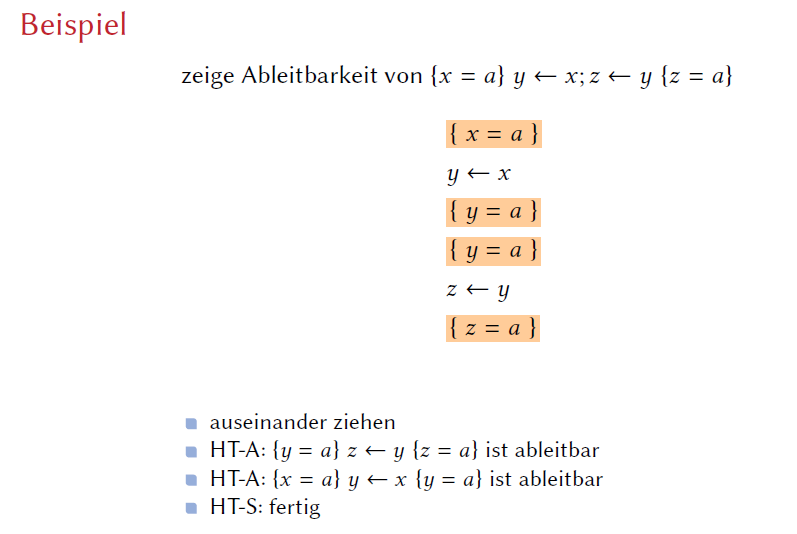
\includegraphics[scale=0.5]{hoare/bsp1}
\end{frame}

\begin{frame}{HT-I}
	\begin{minipage}{0.4\linewidth}
		\begin{align*}
			&\assert{ P } \\
			& \textbf{if } B \textbf{ then} \\
			&\hspace{2em} \assert{ P \wedge B } \\
			&\hspace{2em} S_1 \\
			&\hspace{2em} \assert{ Q }\\
			&\textbf{else} \\
			&\hspace{2em} \assert{ P \wedge \neg B } \\
			&\hspace{2em} S_2 \\
			&\hspace{2em} \assert{ Q }  \\
			&\textbf{fi}\\
			&\assert{Q }
		\end{align*}
	\end{minipage}
	\begin{minipage}{0.55\linewidth}
		\begin{block}{Regel HT-I \quad „If“}
			$\textbf{if } B\text{ } \textbf{ then } S_1 \textbf{ else } S_2 \textbf{ fi}$
			\smallskip
			\begin{itemize}
				\item Wenn $\{ P \wedge B \}\ S_1\ \{ Q \}$ gültig 
				\item und $\{ P \wedge \neg B \}\ S_2\ \{ Q \}$ gültig
				\item dann auch \\ $\{ P \} \textbf{ if } B \textbf{ then } S_1 \textbf{ else } S_2 \textbf{ fi } \{ Q \} $ gültig
			\end{itemize}
		\end{block}
%		\emph{HT4 : } $\textbf{if } B\text{ } \textbf{then } S_1 \textbf{ else } S_2 \textbf{ fi}$
%		\begin{itemize}
%			\item Wenn $\{ P \wedge B \} S_1 \{ Q \}$ gültig 
%			\item Wenn $\{ P \wedge \neg B \} S_2 \{ Q \}$ gültig
%			\item dann auch $\{ P \} \textbf{ if } B \textbf{ then } S_1 \textbf{ else } S_2 \textbf{ fi} \{ Q \} $ gültig
%		\end{itemize}
	\end{minipage}
\end{frame}

\begin{frame}{Beispiel: Berechnung von $\vert x \vert$}
	
	
	\begin{minipage}{0.4\linewidth}
		Erinnerung:
		\vspace{-.6\baselineskip}
		\begin{align*}
		&\assert{ P } \\
		& \textbf{if } B \textbf{ then} \\
		&\hspace{2em} \assert{ P \wedge B } \\
		&\hspace{2em} S_1 \\
		&\hspace{2em} \assert{ Q }\\
		&\textbf{else} \\
		&\hspace{2em} \assert{ P \wedge \neg B } \\
		&\hspace{2em} S_2 \\
		&\hspace{2em} \assert{ Q }  \\
		&\textbf{fi}\\
		&\assert{Q }
		\end{align*}
	\end{minipage}
	\begin{minipage}{0.4\linewidth}
		\begin{align*}
		&\assert{ x \in\R} \\
		&\textbf{if } x < 0 \textbf{ then } \\
		&\hspace{2em} \assert{ \visible<6->{ x\in\R\wedge x < 0 } } \\
		&\hspace{2em} \assert{ \visible<5->{ {-x} = \vert x \vert } } \\
		&\hspace{2em}  z \gets -x   \\
		&\hspace{2em} \assert{ \visible<2->{ z = \vert x \vert } } \\
		&\textbf{else} \\
		&\hspace{2em} \assert{ \visible<4->{ x\in\R\wedge x\geq 0 } } \\
		&\hspace{2em} \assert{ \visible<3->{ x = \vert x \vert } } \\
		&\hspace{2em} z \gets x \\
		&\hspace{2em} \assert{ \visible<2->{ z = \vert x \vert } } \\
		&\textbf{fi} \\
		&\assert{ z = \vert x \vert } 
		\end{align*}
	\end{minipage}
\end{frame}

\begin{frame}{Aufgabe}
	\vspace{-10mm}
	\begin{align*}
	&\assert{x=a \land y=b}  \\
	&\kw{if } x>y \kw{ then } \\
	&\hspace{2em} \assert{ \dots\ } \\
	&\hspace{2em}  z \gets y  \\
	&\hspace{2em} \assert{ \dots\ } \\
	&\kw{else } \\
	&\hspace{2em} \assert{ \dots\ } \\
	&\hspace{2em}  z \gets x  \\
	&\hspace{2em} \assert{ \dots\ } \\
	&\kw{fi } \\
	&\assert{z=\min(a,b)}
	\end{align*}
\end{frame}

\begin{frame}{Lösung}	
	\vspace{-2.5\baselineskip}
	\begin{alignat*}{2}
	&\assert{x=a \land y=b}  \\
	&\kw{if } x>y \kw{ then } \\
	&\hspace{2em} \assert{x=a \land y=b \land x>y} \\
	&\hspace{2em} \assert{y=\min(a,b)} \\
	&\hspace{2em}  z \gets y  \\
	&\hspace{2em} \assert{z=\min(a,b)} \\
	&\kw{else } \\
	&\hspace{2em} \assert{x=a \land y=b \land  \lnot (x>y)} \\
	&\hspace{2em} \assert{x=\min(a,b)} \\
	&\hspace{2em}  z \gets x  \\
	&\hspace{2em} \assert{z=\min(a,b)} \\
	&\kw{fi } \\
	&\assert{z=\min(a,b)}
	\end{alignat*}
\end{frame}


\mycomment{
%TODO: Lösung!!!
\begin{frame}{Jetzt seid ihr dran}
	\begin{align*}
	& z \gets x + y \\
	& z \gets z / 2 \\
	&\textbf{if } x \mod 2 = 0 \textbf{ then } \\
	&\hspace{2em} y \gets x + x \\
	&\hspace{2em} y \gets y / 4 \\
	&\textbf{else} \\
	&\hspace{2em} y \gets x - 1 \\
	&\hspace{2em} y \gets y / 2 \\
	&\textbf{fi} \\
	& z \gets z \· y \\
	&\assert{ z = div_2(a) \· (a+b)/2 } % WTF is div_2 ? => (2 `div`) ? a, b vs. x, y?
	\end{align*}
\end{frame}	
}


%\begin{frame}
%	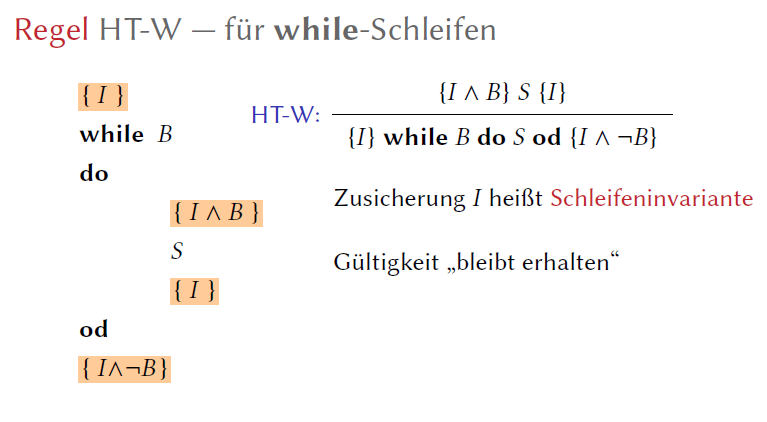
\includegraphics[scale=0.5]{hoare/htw}
%\end{frame}

\subsection{HT-W, Schleifeninvarianten}
\begin{frame}{HT-W}
	\begin{columns}[T] 
		\begin{column}[T]{.4\textwidth} 
			\vspace{-2\baselineskip}
			\begin{align*}
			&\assert{I} \q3uad \text{„Schleifeninvariante“} \\
			&\kw{while } B \kw{ do } \\
			&\qquad \assert{I \land B} \\
			&\qquad S \\
			&\qquad \assert{I} \\
			&\kw{od} \\
			&\assert{I \land \lnot B}
			\end{align*}
			\vspace{-1\baselineskip}
		\end{column}
		\begin{column}[T]{.4\textwidth} 
			\begin{block}{Regel HT-W \quad „While“}
				Wenn \htr{$I \land B$}{$S$}{$I$} gültig ist, dann ist auch die ganze \kw{while}-Schleife (s. links) gültig
			\end{block}
		\end{column}
	\end{columns}
	
	\pause
	\begin{block}{Schleifeninvarianten}
		\begin{itemize}
			\item sind Aussagen, die zu Beginn und Ende jedes Schleifendurchganges gültig sind
			\item helfen, die Korrektheit eines Programmes zu beweisen
			\item muss man ebenfalls beweisen 
			\item garantieren nicht die Korrektheit des Programms:\pause \\
			Terminierung der Schleife muss zusätzlich gezeigt werden! (nicht in GBI)
		\end{itemize}
	\end{block}
\end{frame}
	
\begin{frame}{Beispiel Schleifeninvarianten}
	\begin{columns}
	\begin{column}[T]{0.49\linewidth}
	\begin{align*}
		&\assert{x=a \land y=b}  \\
		&\assert{ \dots\ } \\
		&\kw{while } y\not=0 \kw{ do } \\
		&\qquad\assert{ \dots } \\
		&\qquad y \gets y-1 \\
		&\qquad\assert{ \dots } \\
		&\qquad x \gets x+1 \\
		&\qquad\assert{ \dots\ } \\
		&\kw{od } \\
		&\assert{ \dots\ } \\ \pause
		&\assert{x=a+b} \\
	\end{align*}
	\end{column} 
	
	\begin{column}[T]{0.5\linewidth}
		\visible<2->{
			\bigskip
			\begin{block}{Wertetabelle für $a=3$ und $b=4$}
				\centering
				\medskip
				\begin{tabular}{c|cc}	 
					Durchlauf $i$ & $x$ & $y$ \\ 
					\hline 
					0 & 3 & 4 \\
					1 & 4 & 3 \\
					2 & 5 & 2 \\
					3 & 6 & 1 \\
					4 & 7 & 0 \\
				\end{tabular}
			\end{block}
			\pause
			Schleifeninvariante: $$ x + y = a + b $$ 
		}
	\end{column}
	\end{columns}
\end{frame}

\begin{frame}{Beispiel Schleifeninvarianten – Lösung}
	\begin{minipage}{.4\linewidth}
		Erinnerung HT-W:
		\vspace{-.4\baselineskip}
		\begin{align*}
		&\assert{I}  \\
		&\kw{while } B \kw{ do } \\
		&\qquad \assert{I \land B} \\
		&\qquad S \\
		&\qquad \assert{I} \\
		&\kw{od} \\
		&\assert{I \land \lnot B}
		\end{align*}
	\end{minipage}
	\begin{minipage}{.4\linewidth}
		\begin{align*}
		&\assert{x=a \land y=b }  \\
		&\assert{ x+y=a+b }  \\
		&\kw{while } y\not=0 \kw{ do } \\
		&\qquad\assert{x+y=a+b \land y\not=0 }  \\
		&\qquad\assert{x+1+y-1=a+b } \\
		&\qquad y \gets y-1 \\
		&\qquad\assert{x+1+y = a+b} \\
		&\qquad x \gets x+1 \\
		&\qquad\assert{ x+y = a+b} \\
		&\kw{od } \\
		&\assert{ x+y = a+b \land y=0 } \\
		&\assert{x=a+b} \\
		\end{align*}
	\end{minipage}
	
\end{frame}

\begin{frame}{Exkurs: Schl.-Inv. mit Vollst. Induktion}
	Wir zeigen mit vollständiger Induktion die Gültigkeit der Schleifeninvariante. Dabei sei $i$ die Anzahl der bisher durchgelaufenen Schleifendurchläufe.\\
	
	\emph{Behauptung}: $$ \forall\ i \in \{0,...,b\} : x_i + y_i = a+b $$ \pause
	\begin{block}{Induktionsanfang}
		Für $i=0$ gilt $ x_0+y_0 = a+b $ nach Vorbedingung.
	\end{block} \pause 
	\begin{block}{Induktionsvorrausetzung}
		Für ein beliebig aber festes $i\in \{0,...,b\}$ gelte die Behauptung.
	\end{block}
\end{frame}

\begin{frame}{Exkurs: Schl.-Inv. mit Vollst. Induktion}
	\vspace{-2\baselineskip}
	\begin{align*}
	&\assert{x=a \land y=b}  \\
	&\assert{ x+y=a+b }\\
	&\kw{while } y\not=0 \kw{ do } \\
	&\qquad y \gets y-1 \\
	&\qquad x \gets x+1 \\
	&\kw{od } \\
	&\assert{x=a+b} \\
	\end{align*}
	\vspace{-2\baselineskip}
	\begin{block}{Induktionsschluss}
		Zu zeigen: $ x_{i+1} + y_{i+1} = a+b $ \pause
	%\vspace{-1.3\baselineskip}
		\begin{align*}
		x_{i+1}+y_{i+1} &= x_i +1 + y_i -1 \\
		&= x_i + y_i \\
		&\overset{IV}{=} a+b.
		\end{align*}
	\end{block}
\end{frame}

\begin{frame} {Weitere Beispiele}
	Weitere Beispiele findet ihr hier: Übung 8, WS 15/16
\end{frame}
}{
%	\renewcommand{\assert}[1]{\hoareassert{#1}}
\renewcommand{\kw}[1]{\textbf{#1}}

\section{Algorithmen: Hoare-Kalkül}

\subsection{Algorithmen}
\mycomment{%in last tut
	\begin{frame}{Algorithmen}
		\begin{block}{Definition}
			Ein Algorithmus ist...
			\begin{itemize}[<+->]
				\item Eine endliche Beschreibung
				\item aus elementaren Anweisungen, 
				\item die deterministisch ($=$ ohne Zufall!) ausgeführt werden.\\
					{\small (Manchmal auch gemischt mit (Pseudo-)Zufallselementen)}
				\item Eine endliche Eingabe gibt endliche Ausgabe...
				\item in endlich vielen Schritten.
				\item Das funktioniert für beliebig große Eingaben und
				\item ist nachvollziehbar bzw. verständlich.
			\end{itemize}
		\end{block}
		\pause[8]
		Woher wissen wir, ob ein Algorithmus korrekt ist?
	\end{frame}

	\begin{frame}{Korrektheit}
		Einige Algorithmen haben besonders hohe Anforderungen an ihre Korrektheit:
		Banking-Server, Airbag-Steuerprogramm, Herzschrittmacher, ...
		\bigskip

		
		Korrektheit garantieren?\pause
		\begin{itemize}
			\item Testen? \pause Was, wenn wir einen Sonderfall vergessen? \pause
			\item Alle Eingaben testen? \pause Oft nicht möglich. \pause
			\item Formal beweisen: \textbf{Hoare-Kalkül} \pause
		\end{itemize}
		
		\begin{block}{In der Praxis}
			Theoretisch müsste die komplette Werkzeugkette bewiesen werden:
			Programm, Compiler, Prozessor...\\
			Oft wird bei Compilern nur “Proven in use” benutzt: Compiler, bei
			denen seit Jahren keine Fehler gefunden wurden.
		\end{block}
		
	\end{frame}
}
\subsection{Hoare-Kalkül}
\begin{frame}{Der Hoare-Kalkül}
	\begin{block}{Definition}
		Ein \emph{Hoare-Tripel} ist ein Tripel $\set{P}\ S \ \set{Q}$ mit einem Programmstück $S$ und prädikatenlogischen \emph{Zusicherungen} $P,Q$.
	\end{block}
	\pause
	$P = $ Vorbedingung vor der Ausführung \\
	$Q = $ Nachbedingung nach der Ausführung\\
	$S = $ Programmstück
	
	\pause
	\bigskip
	Dabei: Wir betrachten nur \enquote{relevante} Interpretationen:
	\begin{itemize}[<+->]
		\item Fester Grundbereich (explizit angegeben oder implizit ableitbar)
		\item Funktionen und Relationen \enquote{wie üblich} interpretiert.
		\item Konstanten beliebig, als \enquote{Eingabe} des Programms.\\
		Muss also für alle Möglichkeiten (also Eingaben) gelten.
	\end{itemize}
\end{frame}

%TODO
\begin{frame}{Der Hoare-Kalkül}
	\begin{block}{Definition}
		Ein Hoare-Tripel $\htr{P}{S}{Q}$ ist \textbf{gültig}, wenn für jede relevante Interpretation $I$ und jede Variablenbelegung $\beta$ gilt:\\
		Wenn vor der Ausführung $\val_{D,I,\beta}(P)=\W$ ist und die Ausführung von $S$ für $I$ und $\beta$ mit der neuen Variablenbelegung $\beta'$ endet, dann gilt anschließend auch $\val_{D,I,\beta'}(Q)=\W$. \\
		\medskip
		Auf Deutsch: \\
		$\htr{P}{S}{Q}$ ist \textbf{gültig} \Gdw Wenn anfangs $P$ gilt, wir $S$ ausführen und dann zum Schluss $Q$ gilt.
	\end{block}
\end{frame}

\begin{frame}{Hoare-Tripel}
	\begin{Beispiel}
		\begin{columns}[T] 
			\begin{column}[T]{.4\textwidth} 
				$\assert{x = 5}$ \\
				$x \gets x + 1$ \\
				$\assert{x = 6}$ \\
				ist gültig.  \\
				
				\bigskip
				$\assert{x = 5}$ \\
				$x \gets x + 1$ \\
				$\assert{x = 42}$ \\
				ist nicht gültig.
			\end{column}
			\begin{column}[T]{.4\textwidth} 
				\pause
				$\assert{z = 5}$ \\
				$x \gets x + 1$ \\
				$\assert{z = 5}$ \\
				ist gültig.  \\
				
				
				\bigskip
				$\assert{x = x}$ \\
				$\kw{while } 1 = 1 \kw{ do } x \gets x + 1 \kw{ od}$ \\
				$\assert{\W = \F}$ \\
				ist gültig (Q wird nie erreicht).
			\end{column}
		\end{columns}
	\end{Beispiel}
	\medskip
	\pause
	\begin{block}{Hoare-Kalkül}
		Der \emph{Hoare-Kalkül} definiert Regeln, wie gültige \emph{Hoare-Tripel} schrittweise aus Axiomen abgeleitet werden können.
	\end{block}
\end{frame}


\begin{frame}{HT-A}
	\begin{block} {Axiom HT-A \quad „Assignment“}
		$$ \{\sigma_{\{\text{x/E}\}} (Q)\} \quad x \leftarrow E \quad \{Q\} $$
	\end{block}
	\pause
	Nach einer Zuweisung gilt jede Aussage für die Variable, welche vorher für die rechte Seite der Zuweisung galt.
	\begin{itemize}
		\item $\sigma_{\{\text{x/E}\}} (Q) $ ist die Aussage, die dadurch entsteht, dass man in Q jedes freie Vorkommen von x durch E ersetzt.
		\item \textbf{Achtung}: $\sigma_{\{\text{x/E}\}}$ muss kollisionfrei sein!
	\end{itemize}
	
	\begin{Beispiel}
		$\{ x + 1 = 43\} \ y \gets x + 1\ \{y = 43 \}$ ist gültig. \pause (Bzw. umgeformt \\
		$\{ x = 42 \} \ y \gets x + 1\ \{y = 43 \}$).
	\end{Beispiel}
	
\end{frame}

\begin{frame}{HT-E}
	\begin{block}{Regel HT-E}
		Wenn $\{P\}\ S\ \{Q\}$ gültig ist, dann auch $\{P'\}\ S\ \{Q'\}$ mit $P' \impl P$ und $Q \impl  Q'$.
	\end{block}
	\pause
	Heißt: Vorbedingungen können stärker, Nachbedingungen können schwächer werden.

	\begin{Beispiel}
		Aus $\{ x = 41\} \ x \gets x + 1\ \{x = 42 \}$ können wir \\
		$\{ x + y = 42 \land y = 1 \} \ x \gets x + 1\ \{x \in \R \}$ ableiten.
	\end{Beispiel}
\end{frame}

\begin{frame}{HT-S}
	\begin{block}{Regel HT-S \quad „Sequence“}
		Wenn $\{P\}\ S_1\ \{Q\}$ und $\{Q\}\ S_2\ \{R\}$ gültig sind, dann auch $\{P\}\ S_1;  S_2\ \{R\}$. 
	\end{block}
	\pause
	\impl Hoare-Tripel können transitiv zusammengefasst werden.
\end{frame}

\begin{frame}
	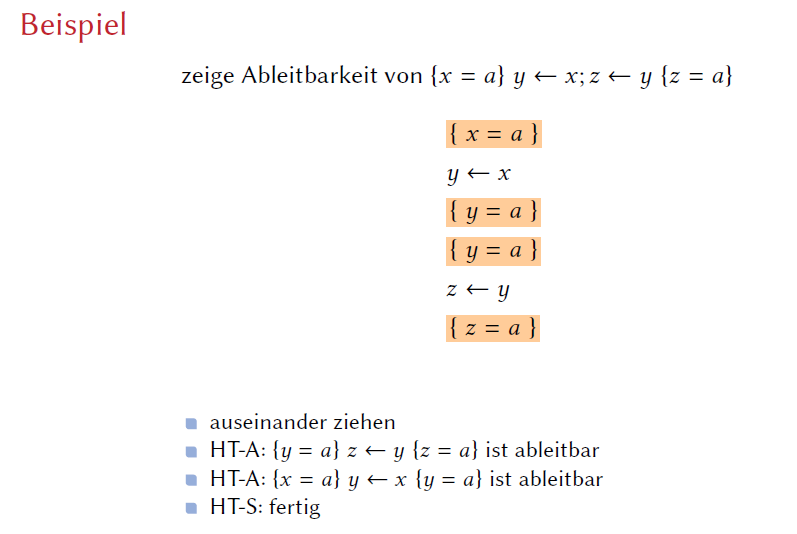
\includegraphics[scale=0.5]{hoare/bsp1}
\end{frame}

\begin{frame}{HT-I}
	\begin{minipage}{0.4\linewidth}
		\begin{align*}
			&\assert{ P } \\
			& \textbf{if } B \textbf{ then} \\
			&\hspace{2em} \assert{ P \wedge B } \\
			&\hspace{2em} S_1 \\
			&\hspace{2em} \assert{ Q }\\
			&\textbf{else} \\
			&\hspace{2em} \assert{ P \wedge \neg B } \\
			&\hspace{2em} S_2 \\
			&\hspace{2em} \assert{ Q }  \\
			&\textbf{fi}\\
			&\assert{Q }
		\end{align*}
	\end{minipage}
	\begin{minipage}{0.55\linewidth}
		\begin{block}{Regel HT-I \quad „If“}
			$\textbf{if } B\text{ } \textbf{ then } S_1 \textbf{ else } S_2 \textbf{ fi}$
			\smallskip
			\begin{itemize}
				\item Wenn $\{ P \wedge B \}\ S_1\ \{ Q \}$ gültig 
				\item und $\{ P \wedge \neg B \}\ S_2\ \{ Q \}$ gültig
				\item dann auch \\ $\{ P \} \textbf{ if } B \textbf{ then } S_1 \textbf{ else } S_2 \textbf{ fi } \{ Q \} $ gültig
			\end{itemize}
		\end{block}
%		\emph{HT4 : } $\textbf{if } B\text{ } \textbf{then } S_1 \textbf{ else } S_2 \textbf{ fi}$
%		\begin{itemize}
%			\item Wenn $\{ P \wedge B \} S_1 \{ Q \}$ gültig 
%			\item Wenn $\{ P \wedge \neg B \} S_2 \{ Q \}$ gültig
%			\item dann auch $\{ P \} \textbf{ if } B \textbf{ then } S_1 \textbf{ else } S_2 \textbf{ fi} \{ Q \} $ gültig
%		\end{itemize}
	\end{minipage}
\end{frame}

\begin{frame}{Beispiel: Berechnung von $\vert x \vert$}
	
	
	\begin{minipage}{0.4\linewidth}
		Erinnerung:
		\vspace{-.6\baselineskip}
		\begin{align*}
		&\assert{ P } \\
		& \textbf{if } B \textbf{ then} \\
		&\hspace{2em} \assert{ P \wedge B } \\
		&\hspace{2em} S_1 \\
		&\hspace{2em} \assert{ Q }\\
		&\textbf{else} \\
		&\hspace{2em} \assert{ P \wedge \neg B } \\
		&\hspace{2em} S_2 \\
		&\hspace{2em} \assert{ Q }  \\
		&\textbf{fi}\\
		&\assert{Q }
		\end{align*}
	\end{minipage}
	\begin{minipage}{0.4\linewidth}
		\begin{align*}
		&\assert{ x \in\R} \\
		&\textbf{if } x < 0 \textbf{ then } \\
		&\hspace{2em} \assert{ \visible<6->{ x\in\R\wedge x < 0 } } \\
		&\hspace{2em} \assert{ \visible<5->{ {-x} = \vert x \vert } } \\
		&\hspace{2em}  z \gets -x   \\
		&\hspace{2em} \assert{ \visible<2->{ z = \vert x \vert } } \\
		&\textbf{else} \\
		&\hspace{2em} \assert{ \visible<4->{ x\in\R\wedge x\geq 0 } } \\
		&\hspace{2em} \assert{ \visible<3->{ x = \vert x \vert } } \\
		&\hspace{2em} z \gets x \\
		&\hspace{2em} \assert{ \visible<2->{ z = \vert x \vert } } \\
		&\textbf{fi} \\
		&\assert{ z = \vert x \vert } 
		\end{align*}
	\end{minipage}
\end{frame}

\begin{frame}{Aufgabe}
	\vspace{-10mm}
	\begin{align*}
	&\assert{x=a \land y=b}  \\
	&\kw{if } x>y \kw{ then } \\
	&\hspace{2em} \assert{ \dots\ } \\
	&\hspace{2em}  z \gets y  \\
	&\hspace{2em} \assert{ \dots\ } \\
	&\kw{else } \\
	&\hspace{2em} \assert{ \dots\ } \\
	&\hspace{2em}  z \gets x  \\
	&\hspace{2em} \assert{ \dots\ } \\
	&\kw{fi } \\
	&\assert{z=\min(a,b)}
	\end{align*}
\end{frame}

\begin{frame}{Lösung}	
	\vspace{-2.5\baselineskip}
	\begin{alignat*}{2}
	&\assert{x=a \land y=b}  \\
	&\kw{if } x>y \kw{ then } \\
	&\hspace{2em} \assert{x=a \land y=b \land x>y} \\
	&\hspace{2em} \assert{y=\min(a,b)} \\
	&\hspace{2em}  z \gets y  \\
	&\hspace{2em} \assert{z=\min(a,b)} \\
	&\kw{else } \\
	&\hspace{2em} \assert{x=a \land y=b \land  \lnot (x>y)} \\
	&\hspace{2em} \assert{x=\min(a,b)} \\
	&\hspace{2em}  z \gets x  \\
	&\hspace{2em} \assert{z=\min(a,b)} \\
	&\kw{fi } \\
	&\assert{z=\min(a,b)}
	\end{alignat*}
\end{frame}


\mycomment{
%TODO: Lösung!!!
\begin{frame}{Jetzt seid ihr dran}
	\begin{align*}
	& z \gets x + y \\
	& z \gets z / 2 \\
	&\textbf{if } x \mod 2 = 0 \textbf{ then } \\
	&\hspace{2em} y \gets x + x \\
	&\hspace{2em} y \gets y / 4 \\
	&\textbf{else} \\
	&\hspace{2em} y \gets x - 1 \\
	&\hspace{2em} y \gets y / 2 \\
	&\textbf{fi} \\
	& z \gets z \· y \\
	&\assert{ z = div_2(a) \· (a+b)/2 } % WTF is div_2 ? => (2 `div`) ? a, b vs. x, y?
	\end{align*}
\end{frame}	
}


%\begin{frame}
%	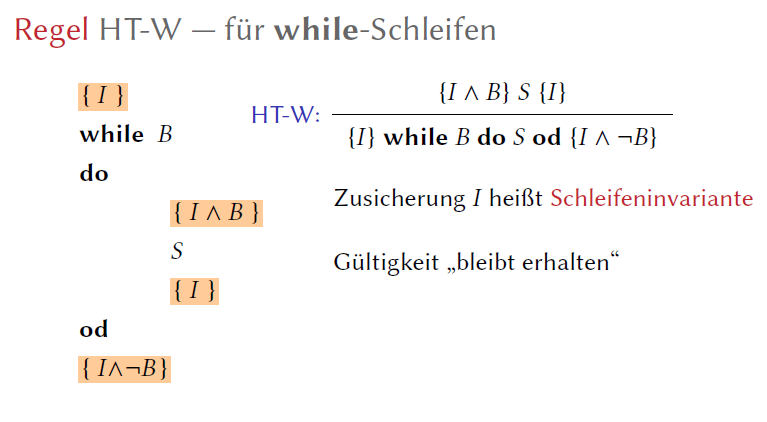
\includegraphics[scale=0.5]{hoare/htw}
%\end{frame}

\subsection{HT-W, Schleifeninvarianten}
\begin{frame}{HT-W}
	\begin{columns}[T] 
		\begin{column}[T]{.4\textwidth} 
			\vspace{-2\baselineskip}
			\begin{align*}
			&\assert{I} \q3uad \text{„Schleifeninvariante“} \\
			&\kw{while } B \kw{ do } \\
			&\qquad \assert{I \land B} \\
			&\qquad S \\
			&\qquad \assert{I} \\
			&\kw{od} \\
			&\assert{I \land \lnot B}
			\end{align*}
			\vspace{-1\baselineskip}
		\end{column}
		\begin{column}[T]{.4\textwidth} 
			\begin{block}{Regel HT-W \quad „While“}
				Wenn \htr{$I \land B$}{$S$}{$I$} gültig ist, dann ist auch die ganze \kw{while}-Schleife (s. links) gültig
			\end{block}
		\end{column}
	\end{columns}
	
	\pause
	\begin{block}{Schleifeninvarianten}
		\begin{itemize}
			\item sind Aussagen, die zu Beginn und Ende jedes Schleifendurchganges gültig sind
			\item helfen, die Korrektheit eines Programmes zu beweisen
			\item muss man ebenfalls beweisen 
			\item garantieren nicht die Korrektheit des Programms:\pause \\
			Terminierung der Schleife muss zusätzlich gezeigt werden! (nicht in GBI)
		\end{itemize}
	\end{block}
\end{frame}
	
\begin{frame}{Beispiel Schleifeninvarianten}
	\begin{columns}
	\begin{column}[T]{0.49\linewidth}
	\begin{align*}
		&\assert{x=a \land y=b}  \\
		&\assert{ \dots\ } \\
		&\kw{while } y\not=0 \kw{ do } \\
		&\qquad\assert{ \dots } \\
		&\qquad y \gets y-1 \\
		&\qquad\assert{ \dots } \\
		&\qquad x \gets x+1 \\
		&\qquad\assert{ \dots\ } \\
		&\kw{od } \\
		&\assert{ \dots\ } \\ \pause
		&\assert{x=a+b} \\
	\end{align*}
	\end{column} 
	
	\begin{column}[T]{0.5\linewidth}
		\visible<2->{
			\bigskip
			\begin{block}{Wertetabelle für $a=3$ und $b=4$}
				\centering
				\medskip
				\begin{tabular}{c|cc}	 
					Durchlauf $i$ & $x$ & $y$ \\ 
					\hline 
					0 & 3 & 4 \\
					1 & 4 & 3 \\
					2 & 5 & 2 \\
					3 & 6 & 1 \\
					4 & 7 & 0 \\
				\end{tabular}
			\end{block}
			\pause
			Schleifeninvariante: $$ x + y = a + b $$ 
		}
	\end{column}
	\end{columns}
\end{frame}

\begin{frame}{Beispiel Schleifeninvarianten – Lösung}
	\begin{minipage}{.4\linewidth}
		Erinnerung HT-W:
		\vspace{-.4\baselineskip}
		\begin{align*}
		&\assert{I}  \\
		&\kw{while } B \kw{ do } \\
		&\qquad \assert{I \land B} \\
		&\qquad S \\
		&\qquad \assert{I} \\
		&\kw{od} \\
		&\assert{I \land \lnot B}
		\end{align*}
	\end{minipage}
	\begin{minipage}{.4\linewidth}
		\begin{align*}
		&\assert{x=a \land y=b }  \\
		&\assert{ x+y=a+b }  \\
		&\kw{while } y\not=0 \kw{ do } \\
		&\qquad\assert{x+y=a+b \land y\not=0 }  \\
		&\qquad\assert{x+1+y-1=a+b } \\
		&\qquad y \gets y-1 \\
		&\qquad\assert{x+1+y = a+b} \\
		&\qquad x \gets x+1 \\
		&\qquad\assert{ x+y = a+b} \\
		&\kw{od } \\
		&\assert{ x+y = a+b \land y=0 } \\
		&\assert{x=a+b} \\
		\end{align*}
	\end{minipage}
	
\end{frame}

\begin{frame}{Exkurs: Schl.-Inv. mit Vollst. Induktion}
	Wir zeigen mit vollständiger Induktion die Gültigkeit der Schleifeninvariante. Dabei sei $i$ die Anzahl der bisher durchgelaufenen Schleifendurchläufe.\\
	
	\emph{Behauptung}: $$ \forall\ i \in \{0,...,b\} : x_i + y_i = a+b $$ \pause
	\begin{block}{Induktionsanfang}
		Für $i=0$ gilt $ x_0+y_0 = a+b $ nach Vorbedingung.
	\end{block} \pause 
	\begin{block}{Induktionsvorrausetzung}
		Für ein beliebig aber festes $i\in \{0,...,b\}$ gelte die Behauptung.
	\end{block}
\end{frame}

\begin{frame}{Exkurs: Schl.-Inv. mit Vollst. Induktion}
	\vspace{-2\baselineskip}
	\begin{align*}
	&\assert{x=a \land y=b}  \\
	&\assert{ x+y=a+b }\\
	&\kw{while } y\not=0 \kw{ do } \\
	&\qquad y \gets y-1 \\
	&\qquad x \gets x+1 \\
	&\kw{od } \\
	&\assert{x=a+b} \\
	\end{align*}
	\vspace{-2\baselineskip}
	\begin{block}{Induktionsschluss}
		Zu zeigen: $ x_{i+1} + y_{i+1} = a+b $ \pause
	%\vspace{-1.3\baselineskip}
		\begin{align*}
		x_{i+1}+y_{i+1} &= x_i +1 + y_i -1 \\
		&= x_i + y_i \\
		&\overset{IV}{=} a+b.
		\end{align*}
	\end{block}
\end{frame}

\begin{frame} {Weitere Beispiele}
	Weitere Beispiele findet ihr hier: Übung 8, WS 15/16
\end{frame}
%	\input{../Bloecke/DrMetaNordpol}
}

\begin{frame}	
	\begin{block}{Was ihr nun wissen solltet}
		\begin{itemize}
			\item Wie Prädikatenlogische Formeln aufgebaut sind
			\item Wie man damit präzise Aussagen trifft
			\item Wie man sie auswertet
			%\item Wie der Hoare-Kalkül funktioniert % TODO maybe
			%\item Wie man mit dem Hoare-Kalkül ein Programm beweist.
		\end{itemize}
	\end{block}
	
	\begin{block}{Was nächstes Mal kommt}
		\begin{itemize}
			\item Alles korrekt? –- Beweise mit dem Hoare-Kalkül
			\item Graphen -- Alles vernetzt
			\item Systematisches Suchen und Wandern -- Algorithmen auf Graphen
		\end{itemize}
	\end{block}
\end{frame}

%\xkcdframevert{835}{Frohe Weihnachten und bis nächstes Jahr! \smiley}{2.2}
%\lastframetitled{0.47}{0}{xkcd/christmastree.png}{https://www.xkcd.com/835}{\vspace{-1.66\baselineskip}\\Frohe Weihnachten und einen \\ guten Start ins neue Jahr! \smiley}
\slideThanks

\end{document}